\documentclass{beamer}
\usepackage[utf8]{inputenc}

\usetheme{Madrid}
\usecolortheme{default}
\usepackage{amsmath,amssymb,amsfonts,amsthm}
\usepackage{txfonts}
\usepackage{tkz-euclide}
\usepackage{listings}
\usepackage{adjustbox}
\usepackage{array}
\usepackage{tabularx}
\usepackage{gvv}
\usepackage{lmodern}
\usepackage{circuitikz}
\usepackage{tikz}
\usepackage{graphicx}

\setbeamertemplate{page number in head/foot}[totalframenumber]

\usepackage{tcolorbox}
\tcbuselibrary{minted,breakable,xparse,skins}



\definecolor{bg}{gray}{0.95}
\DeclareTCBListing{mintedbox}{O{}m!O{}}{%
  breakable=true,
  listing engine=minted,
  listing only,
  minted language=#2,
  minted style=default,
  minted options={%
    linenos,
    gobble=0,
    breaklines=true,
    breakafter=,,
    fontsize=\small,
    numbersep=8pt,
    #1},
  boxsep=0pt,
  left skip=0pt,
  right skip=0pt,
  left=25pt,
  right=0pt,
  top=3pt,
  bottom=3pt,
  arc=5pt,
  leftrule=0pt,
  rightrule=0pt,
  bottomrule=2pt,

  colback=bg,
  colframe=orange!70,
  enhanced,
  overlay={%
    \begin{tcbclipinterior}
    \fill[orange!20!white] (frame.south west) rectangle ([xshift=20pt]frame.north west);
    \end{tcbclipinterior}},
  #3,
}
\lstset{
    language=C,
    basicstyle=\ttfamily\small,
    keywordstyle=\color{blue},
    stringstyle=\color{orange},
    commentstyle=\color{green!60!black},
    numbers=left,
    numberstyle=\tiny\color{gray},
    breaklines=true,
    showstringspaces=false,
}
%------------------------------------------------------------
%This block of code defines the information to appear in the
%Title page
\title %optional
{2.7.3}
\date{\today}
%\subtitle{A short story}

\author % (optional)
{Shivam Sawarkar \\ AI25BTECH11031}



\begin{document}


\frame{\titlepage}
\begin{frame}{Question (2.7.3)}
If $\vec{a}$ and $\vec{b}$ are two vectors such that $\vec{a} = \hat{i} - \hat{j} + \hat{k}$, $\vec{b} = 2\hat{i} - \hat{j} - 3\hat{k}$, then find the vector $\vec{c}$, given that $\vec{a} \times \vec{c} = \vec{b}$, $\vec{a} \cdot \vec{c} = 4$.
\end{frame}

\begin{frame}{Solution}
\begin{align}
\vec{a} = \myvec{1 \\ -1 \\ 1} \quad 
\vec{b} = \myvec{2 \\ -1 \\ -3} \quad 
\vec{c} = \myvec{c_1 \\ c_2 \\ c_3}
\end{align}

\begin{align}
\vec{a}\times\vec{c} = \vec{b} \\ 
\implies \vec{c} \perp \vec{b} \\ 
\therefore \vec{b}^\top\vec{c}=0
\end{align}
\end{frame}

\begin{frame}{Solution}
    and $\vec{a}^\top\vec{c}=4$ is given

\begin{align}
    \myvec{\vec{a} & \vec{b}}^\top\vec{c}=\myvec{4 \\ 0} \\ 
    \myvec{1 & -1 & 1 \\ 
           2 & -1 & -3}\vec{c}=\myvec{4 \\ 0} \\ 
    \myvec{1 & -1 & 1 \\ 
    2 & -1 & -3}\myvec{c_1 \\ c_2 \\ c_3}= \myvec{4 \\ 0}
\end{align}
Let, $c_3=\lambda$ \\
Then 
\begin{align}
c_1=-4+4\lambda \\ 
c_2=-8+5\lambda
\end{align}
\end{frame}

\begin{frame}{Solution}
\begin{align}
    \vec{c}=\myvec{-4 \\ -8 \\ 0}+\lambda\myvec{4 \\ 5 \\ 1}
\end{align}
This satisfies all the given conditions when $\lambda=1$ \\ Thus,
\begin{align}
    \vec{c}=\myvec{0 \\ -3 \\ 1}
\end{align}
\end{frame}

\begin{frame}{Plot}
    \begin{figure}
        \centering
        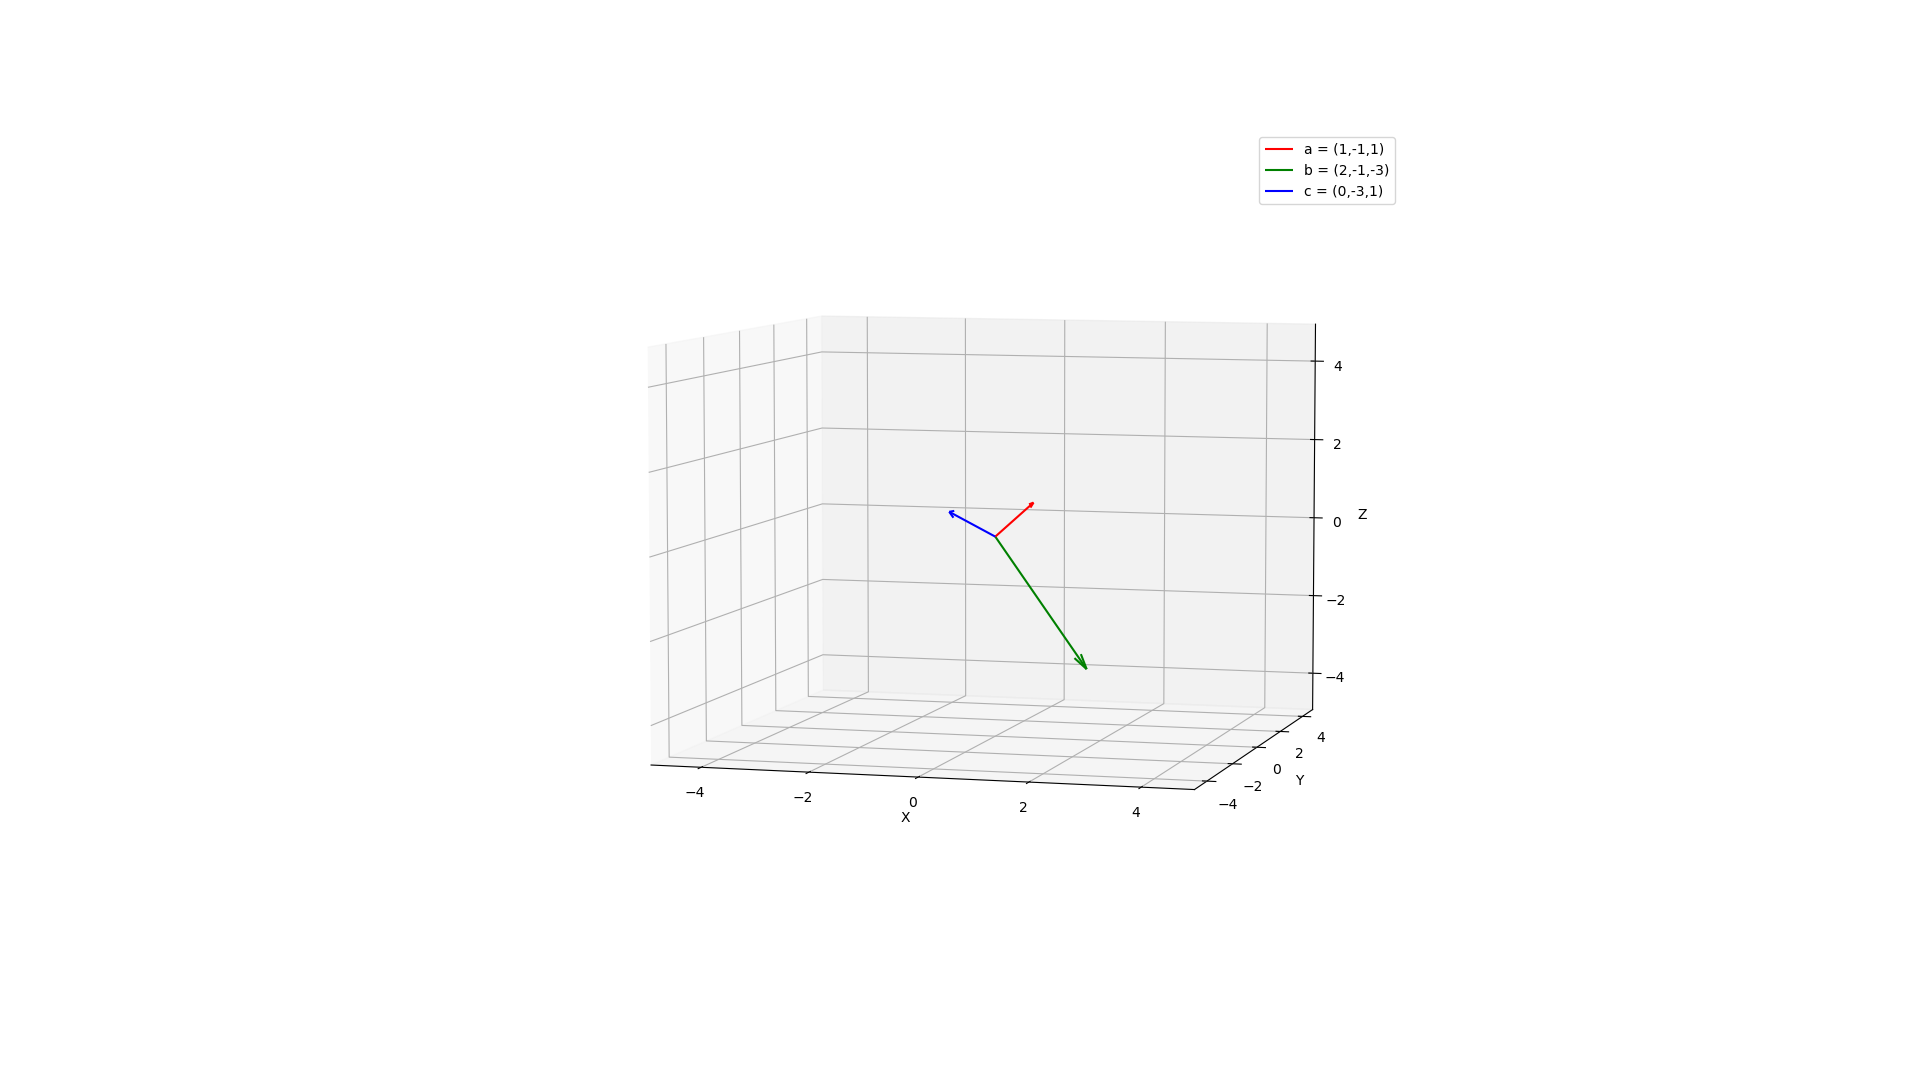
\includegraphics[width=1\columnwidth]{figs/plot4.png}
        \caption{}
        \label{fig:placeholder}
    \end{figure}
\end{frame}

\begin{frame}[fragile]{C Code}
    \begin{verbatim}
#ifndef VECTOR_UTILS_H
#define VECTOR_UTILS_H

// Cross product of 3D vectors
void cross_product(double a[3], double b[3], double result[3]) {
    result[0] = a[1]*b[2] - a[2]*b[1];
    result[1] = a[2]*b[0] - a[0]*b[2];
    result[2] = a[0]*b[1] - a[1]*b[0];
}

// Dot product of 3D vectors
double dot_product(double a[3], double b[3]) {
    return a[0]*b[0] + a[1]*b[1] + a[2]*b[2];
}
\end{verbatim}
\end{frame}

\begin{frame}[fragile]{C Code}
    \begin{verbatim}
// Compute vector c = (a*k - (a×b)) / (||a||^2)
void compute_c(double a[3], double b[3], double k, double c[3]) {
    double cross[3];
    cross_product(a, b, cross);

    double norm_sq = dot_product(a, a); // |a|^2

    for (int i = 0; i < 3; i++) {
        c[i] = (a[i]*k - cross[i]) / norm_sq;
    }
}

#endif
    \end{verbatim}
\end{frame}

\begin{frame}[fragile]{C Code}
    \begin{verbatim}
#include <stdio.h>
#include "solution.h"

int main() {
    double a[3], b[3], c[3], k;
    printf("Enter vector a (3 values): ");
    scanf("%lf %lf %lf", &a[0], &a[1], &a[2]);
    printf("Enter vector b (3 values): ");
    scanf("%lf %lf %lf", &b[0], &b[1], &b[2]);
    printf("Enter scalar k (a·c): ");
    scanf("%lf", &k);
    compute_c(a, b, k, c);
    printf("\nVector c = (%.2lf, %.2lf, %.2lf)\n", c[0], c[1], c[2]);
    return 0;
}
    \end{verbatim}
\end{frame}

\begin{frame}[fragile]{Python + C Code}
    \begin{verbatim}
import ctypes
import numpy as np

# Load shared library
lib = ctypes.CDLL("./solution.so")

# Define argument and return types
lib.compute_c.argtypes = [
    ctypes.POINTER(ctypes.c_double),
    ctypes.POINTER(ctypes.c_double),
    ctypes.c_double,
    ctypes.POINTER(ctypes.c_double),
]
\end{verbatim}
\end{frame}

\begin{frame}[fragile]{Python + C Code}
    \begin{verbatim}
def compute_c(a, b, k):
    a_arr = (ctypes.c_double * 3)(*a)
    b_arr = (ctypes.c_double * 3)(*b)
    c_arr = (ctypes.c_double * 3)()
    lib.compute_c(a_arr, b_arr, ctypes.c_double(k), c_arr)
    return np.array([c_arr[0], c_arr[1], c_arr[2]])

a = list(map(float, input("Enter vector a (3 numbers separated by space): ").split()))
b = list(map(float, input("Enter vector b (3 numbers separated by space): ").split()))
k = float(input("Enter scalar k: "))
c = compute_c(a, b, k)

print("Computed c =", c)
    \end{verbatim}
\end{frame}

\begin{frame}[fragile]{Python Code}
    \begin{verbatim}
import numpy as np

def compute_c_from_a_b_k(a, b, k, tol=1e-9):
    a = np.array(a, dtype=float)
    b = np.array(b, dtype=float)

    if np.linalg.norm(a) < tol:
        raise ValueError("Vector a is (nearly) zero — no unique solution.")
    # For b = a x c, b must be perpendicular to a:
    if abs(np.dot(a, b)) > 1e-8:
        raise ValueError("Inconsistent input: a·b must be 0 for b = a × c.")

    a_cross_b = np.cross(a, b)
    denom = np.dot(a, a)   # |a|^2, guaranteed > 0 here
    c = (a * k - a_cross_b) / denom
    return c
    \end{verbatim}
\end{frame}

\begin{frame}[fragile]{Python Code}
    \begin{verbatim}
def parse_vec(s):
    vals = list(map(float, s.strip().split()))
    if len(vals) != 3:
        raise ValueError("Please enter exactly 3 numbers for a vector.")
    return vals
def main():
    try:
        a = parse_vec(input("Enter vector a (3 values separated by space): "))
        b = parse_vec(input("Enter vector b (3 values separated by space): "))
        k = float(input("Enter the value of a·c (scalar k): "))
        c = compute_c_from_a_b_k(a, b, k)
    except Exception as e:
        print("Error:", e)
        return
    print("\nComputed c =", c)
if __name__ == "__main__":
    main()
    \end{verbatim}
\end{frame}




\end{document}